%

\documentclass{beamer}
    
    %    \usepackage[english]{babel}
        %\usepackage[latin1]{inputenc}
        %\usepackage[T1]{fontenc}
    
    \mode<presentation>{
      \setbeamertemplate{background canvas}[vertical shading]
      \usetheme{Berkeley}
      \useoutertheme{himinfolines}
    }
      
    \usepackage{ucs}
    \usepackage[utf8]{inputenc}
    \usepackage[english,polutonikogreek,italian,UKenglish,british]{babel}
    \usepackage{graphicx}
    \usepackage{colortbl}
    \usepackage{multicol}
    \usepackage{ulem}
    \usepackage{verbatim}
    \usepackage{alltt}
    \usepackage{ccicons}
    \usepackage{MnSymbol,wasysym}
    \usepackage{tikzsymbols}
    \usepackage{textcomp}
    \usepackage{xmpincl}
    
    \usepackage{parskip}
    \setcounter{nframes}{105}
    \setcounter{nframe}{1}
    \setbeamercovered{dynamic}
    \newenvironment{grcenv}{\begin{otherlanguage}{greek}}{\end{otherlanguage}}
    \newcommand{\g}[1]{\textgreek{#1}}
    \definecolor{darkgreen}{rgb}{0,0.5,0}
    \definecolor{darkblue}{rgb}{0,0,0.5}
    \definecolor{grey}{rgb}{0.5,0.5,0.5}
    \setcounter{tocdepth}{5}
    
    \makeatletter
    
    \makeatother
    %\includexmp{LicencesAndLicensing}
    
    %frame00 metadata
        \title{Codifica TEI - Elementi editoriali e facsimile}
        \author[A.M. Del Grosso]{Angelo Mario Del Grosso \\ \tiny\textit{(Materiale tratto dalle lezioni di R. Rosselli Del Turco)}}
        \institute{\texttt{angelo.delgrosso@ilc.cnr.it} \\\bigskip\textit{CNR-ILC-LicoLab} \\\url{http://licolab.ilc.cnr.it/}}
        \date{Istituto di Linguistica Computazionale ``A. Zampolli'', \today}
        \AtBeginSection[]{
        \begin{frame}<beamer>
        \addtocounter{nframe}{1}
        \footnotesize
        \frametitle{Progress status}
        \tableofcontents[currentsection,hideothersubsections]
        \end{frame}
        }
    
    \begin{document}
    
    \begin{frame}
        \maketitle
    \end{frame}
    
    \begin{frame}
        \frametitle{Sommario della Lezione}
        \tableofcontents
    \end{frame}
    
    \section{Introduzione agli elementi editoriali e facsimile TEI}
    
    \begin{frame}
        \frametitle{Introduzione Elementi Editoriali}
        \addtocounter{nframe}{1}
        
        %\begin{center}
        %    
\includegraphics[width=.2\textwidth]{../imgs/tei-r.pdf}
        %\end{center}
        \textit{In parte già disponibili nei moduli TEI di base}

        \begin{block}{Elementi per interventi editoriali}
            \emph{Per la critica testuale indispensabili i moduli}
            \begin{itemize}
                \item \textbf{msdescription} \textit{descrizione del manoscritto} 
                \item \textbf{trans} \textit{trascrizione di fonti primarie }
                \item \textbf{textcrit} \textit{apparato critico}
                \item \textbf{gaiji} \textit{caratteri non standard}
            \end{itemize}
        \end{block}
        
    \end{frame}
    
    \begin{frame}
        \frametitle{Introduzione Elementi Editoriali}
        \addtocounter{nframe}{1}
        
        \begin{block}{Altri Moduli Utili}
           \begin{itemize}
               \item \textbf{analysis} \textit{modulo per l'inserimento di semplici analisi e interpretazioni ad elementi con contentuto testuale}
               \item \textbf{certainty} \textit{modulo per la registrazione del grado di "certezza/incertezza" relativo al testo e alla corrispondente marcatura}
               \item \textbf{figures} \textit{modulo per l'inserimento di immagini con relative informazioni}
               \item \textbf{namesdates} \textit{modulo per la codifica dei nomi: persone, luoghi, organizzazioni}
               \item \textbf{verse} \textit{modulo per la codifica di testi poetici}
           \end{itemize}
        \end{block}
        
    \end{frame}
    
    % \begin{frame}
    %     \frametitle{Modularità della TEI}
    %     \addtocounter{nframe}{1}
        
    %    % \begin{center}
    %     % 
\includegraphics[width=.2\textwidth]{../imgs/tei-r.pdf}
    %     % \end{center}
    
    %     \begin{itemize}
            
    %         \item<1-> parleremo del sistema Modulare della TEI
    %             \begin{itemize}
    %                 \item<1-> Moduli
    %                 \item<1-> Classi
    %                 \item<1-> Macro
    %                 \item<1-> Datatype
    %             \end{itemize} 
    %         \item<2-> parleremo degli elementi basilari
    %             \begin{itemize}
    %                 \item<2-> Intestazione TEI (TEIHeader)
    %                 \item<2-> Elementi e attributi presenti in tutti i documenti TEI
    %                 \item<2-> Esempi di codifica
    %             \end{itemize} 
    %     \end{itemize}
        
    % \end{frame}
    
    \section{Elementi editoriali TEI}
    %%
\begin{frame}
    \frametitle{Elementi interventi editoriali}
    \addtocounter{nframe}{1}
    
    %\begin{center}
    %    
\includegraphics[width=.2\textwidth]{../imgs/tei-r.pdf}
    %\end{center}

    \begin{block}{Testo aggiunto, cancellato, lacunoso}
        \begin{itemize}
            \item \texttt{<add>} \textbf{una o più parole aggiunte nel testo}
            \item[] \texttt{questa parola è <add place="supralinear" >stata</add> aggiunta in un secondo momento}
        \end{itemize}
        
    \end{block}
    
\end{frame}

\begin{frame}
    \frametitle{Elementi interventi editoriali}
    \addtocounter{nframe}{1}
    
    %\begin{center}
    %    
\includegraphics[width=.2\textwidth]{../imgs/tei-r.pdf}
    %\end{center}

    \begin{block}{Testo aggiunto, cancellato, lacunoso}
        \begin{itemize}
            \item \texttt{<del>} \textbf{una o più parole cancellate nel testo}
            \item[] \texttt{questa invece era <del rend="overstrike" >era</del> di troppo e l’ho cancellata}
        \end{itemize}
        
    \end{block}
    
\end{frame}


\begin{frame}
    \frametitle{Elementi interventi editoriali}
    \addtocounter{nframe}{1}
    
    %\begin{center}
    %    
\includegraphics[width=.2\textwidth]{../imgs/tei-r.pdf}
    %\end{center}

    \begin{block}{Testo aggiunto, cancellato, lacunoso}
        \begin{itemize}
            \item \texttt{<gap />} \textbf{parte di testo omessa, mancante o illeggibile}
            \item[] \texttt{questa <gap reason="illegible" extent="6" unit="chars"/> è illeggibile (forse "parola"?)}
        \end{itemize}
        
    \end{block}
    
\end{frame}



%%
\begin{frame}
    \frametitle{Elementi interventi editoriali}
    \addtocounter{nframe}{1}
    
    %\begin{center}
    %    
\includegraphics[width=.2\textwidth]{../imgs/tei-r.pdf}
    %\end{center}

    \begin{block}{Testo danneggiato, poco chiaro, inserito dal curatore}
        \begin{itemize}
            \item \texttt{<damage>} \textbf{testo danneggiato nel documento originale}
            \item[] \texttt{per qualche goccia d’acqua questa parola si è <damage agent="water" >scolorita</damage> molto}
        \end{itemize}
        
    \end{block}
    
\end{frame}

\begin{frame}
    \frametitle{Elementi interventi editoriali}
    \addtocounter{nframe}{1}
    
    %\begin{center}
    %    
\includegraphics[width=.2\textwidth]{../imgs/tei-r.pdf}
    %\end{center}

    \begin{block}{Testo danneggiato, poco chiaro, inserito dal curatore}
        \begin{itemize}
            \item \texttt{<unclear>} \textbf{parte di testo interpretabile con difficoltà}
            \item[] \texttt{<unclear reason="faded" >questa</unclear> si legge
            ancora ma con difficoltà}
        \end{itemize}
        
    \end{block}
    
\end{frame}

\begin{frame}
    \frametitle{Elementi interventi editoriali}
    \addtocounter{nframe}{1}
    
    %\begin{center}
    %    
\includegraphics[width=.2\textwidth]{../imgs/tei-r.pdf}
    %\end{center}

    \begin{block}{Testo danneggiato, poco chiaro, inserito dal curatore}
        \begin{itemize}
            \item \texttt{<supplied>} \textbf{testo inserito dal curatore perché illeggibile nell’originale o assente}
            \item[] \texttt{qui <supplied>mancava qualcosa</supplied> nel testo}
        \end{itemize}
        
    \end{block}

    \textit{\texttt{<supplied>}  (fa parte del modulo transcr)}

\end{frame}

%è possibile combinare questi elementi (compreso <gap/>)

%%
\begin{frame}
    \frametitle{Elementi interventi editoriali}
    \addtocounter{nframe}{1}
    
    %\begin{center}
    %    
\includegraphics[width=.2\textwidth]{../imgs/tei-r.pdf}
    %\end{center}

    \begin{block}{Dal Vercelli Book}
         \begin{center}
            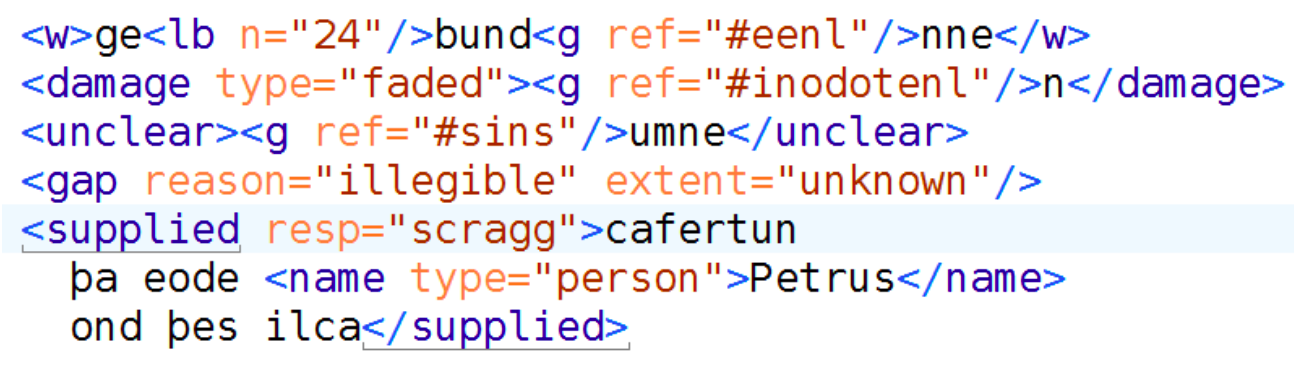
\includegraphics[width=.9\textwidth]{imgs/vercelli.png}
        \end{center}
    \end{block}
    \textit{Manoscritto in inglese antico, dialetto tardo sassone occidentale, X secolo ca.}

\end{frame}
  

%%
\begin{frame}
    \frametitle{Elementi interventi editoriali}
    \addtocounter{nframe}{1}
    
    %\begin{center}
    %    
\includegraphics[width=.2\textwidth]{../imgs/tei-r.pdf}
    %\end{center}

    \begin{block}{Elemento sostituzione}
        Può succedere che una parola non sia semplicemente cancellata, ma che sia anche sostituita da un altro termine
    \end{block}
    \begin{block}{Elemento sostituzione}
        In questo caso è possibile usare l’elemento \texttt{<subst>} per collegare la sequenza cancellazione - nuovo testo
    \end{block}
    \texttt{<subst>} fa parte del modulo transcr, per ulteriori informazioni \texttt{(@seq)} v. \url{http://www.tei-c.org/release/doc/tei-p5-doc/en/html/PH.html\#PHSU}
\end{frame}


%%
\begin{frame}
    \frametitle{Elementi interventi editoriali}
    \addtocounter{nframe}{1}
    
    %\begin{center}
    %    
\includegraphics[width=.2\textwidth]{../imgs/tei-r.pdf}
    %\end{center}

    \begin{block}{Elemento sostituzione: parola}
        \texttt{questa parola è stata <subst> <del rend="overstrike" >scritta</del> <add place="supralinear" >aggiunta</add> </subst> in un secondo momento}
    \end{block}

    \begin{block}{Elemento sostituzione: carattere}
        \texttt{<subst><del rend="overtype" >t<del><add>T</add></subst>i scrivo una     mail domani mattina}
    \end{block}
   
\end{frame}




%%
\begin{frame}
    \frametitle{Elementi interventi editoriali}
    \addtocounter{nframe}{1}
    
    %\begin{center}
    %    
\includegraphics[width=.2\textwidth]{../imgs/tei-r.pdf}
    %\end{center}

    \begin{block}{Attributi e valori consigliati}
        \begin{itemize}
            \item \texttt{<add>} \textbf{place} \textit{inline, supralinear, margin} \textbf{hand} \textit{author, scribe1, scribe2}
            \item \texttt{<del>} \textbf{rend} \textit{overstrike, subpunct, overtype, dotted} \textbf{hand} \textit{author, scribe1, scribe2}
            \item \texttt{<gap>} \textbf{reason} \textit{illegible, cancelled, irrelevant, missing, omissis, censored} \textbf{hand} \textit{editor} \textbf{agent} \textit{water, smoke, hole, missing page} \textbf{extent} \textit{chars, words, cm}
            \item \texttt{<unclear>} \textbf{reason} \textit{parterased, ink blot} \textbf{hand} \textit{author, scribe1, scribe2} \textbf{agent} \textit{water, smoke, ink}
        \end{itemize}
    \end{block}
    
\end{frame}

%%
\begin{frame}
    \frametitle{Elementi interventi editoriali}
    \addtocounter{nframe}{1}
    
    %\begin{center}
    %    
\includegraphics[width=.2\textwidth]{../imgs/tei-r.pdf}
    %\end{center}

    \begin{block}{Correzioni e normalizzazioni}
        \begin{itemize}
            \item \texttt{<sic>} \textbf{parola o frase ritenuta errata, ma riportata così come appare scritta}
            \item[] \texttt{questa parola è <sic>statta</sic> sbagliata}
        \end{itemize}
        
    \end{block}
    
\end{frame}

\begin{frame}
    \frametitle{Elementi interventi editoriali}
    \addtocounter{nframe}{1}
    
    %\begin{center}
    %    
\includegraphics[width=.2\textwidth]{../imgs/tei-r.pdf}
    %\end{center}

    \begin{block}{Correzioni e normalizzazioni}
        \begin{itemize}
            \item \texttt{<corr>} \textbf{correzione di una parola o frase errata}
            \item[] \texttt{questa parola è <corr>stata</corr> corretta in un secondo momento}
        \end{itemize}
        
    \end{block}
    
\end{frame}

\begin{frame}
    \frametitle{Elementi interventi editoriali}
    \addtocounter{nframe}{1}
    
    %\begin{center}
    %    
\includegraphics[width=.2\textwidth]{../imgs/tei-r.pdf}
    %\end{center}

    \begin{block}{Correzioni e normalizzazioni}
        \begin{itemize}
            \item \texttt{<orig>} \textbf{parola o frase ritenuta non standard}
            \item[] \texttt{Allora, mi dici <orig>'ndo</orig> vai?}
        \end{itemize}
        
    \end{block}
    
\end{frame}

\begin{frame}
    \frametitle{Elementi interventi editoriali}
    \addtocounter{nframe}{1}
    
    %\begin{center}
    %    
\includegraphics[width=.2\textwidth]{../imgs/tei-r.pdf}
    %\end{center}

    \begin{block}{Correzioni e normalizzazioni}
        \begin{itemize}
            \item \texttt{<reg>} \textbf{parola o frase normalizzata (regularised)}
            \item[] \texttt{Allora, mi dici <reg>dove</reg> vai?}
        \end{itemize}
        
    \end{block}
    
\end{frame}

%%
\begin{frame}
    \frametitle{Elementi interventi editoriali}
    \addtocounter{nframe}{1}
    
    %\begin{center}
    %    
\includegraphics[width=.2\textwidth]{../imgs/tei-r.pdf}
    %\end{center}

    \begin{block}{Abbreviazioni ed espansioni}
        \begin{itemize}
            \item \texttt{<abbr>} \textbf{parola abbreviata, brevigrafo}
            \item[] \texttt{chiedi al <abbr>dott.</abbr> Rossi}
            \item[] \texttt{in nomine Patris <abbr>7</abbr> Filii
            <abbr>7</abbr> Spiritus Sancti}
        \end{itemize}
        
    \end{block}
    
\end{frame}

\begin{frame}
    \frametitle{Elementi interventi editoriali}
    \addtocounter{nframe}{1}
    
    %\begin{center}
    %    
\includegraphics[width=.2\textwidth]{../imgs/tei-r.pdf}
    %\end{center}

    \begin{block}{Abbreviazioni ed espansioni}
        \begin{itemize}
            \item \texttt{<expan>} \textbf{espansione di un’abbreviazione}
            \item[] \texttt{chiedi al <expan>dottor</expan> Rossi}
            \item[] \texttt{in nomine Patris <expan>et</expan> Filii <expan>et</expan> Spiritus Sancti}
        \end{itemize}
        
    \end{block}
    
\end{frame}

 %%

 \begin{frame}
    \frametitle{Elementi interventi editoriali}
    \addtocounter{nframe}{1}
    
    %\begin{center}
    %    
\includegraphics[width=.2\textwidth]{../imgs/tei-r.pdf}
    %\end{center}

    \begin{block}{Abbreviazioni ed espansioni}
        \begin{itemize}
            \item \texttt{<abbr>} \textbf{usare l’attributo type per specificare il tipo}
            \item[] \texttt{chiedi al <abbr type="titolo" >dott.</abbr> Rossi}
            \item[] \texttt{in nomine Patris <abbr type="brevigrafo" >7</abbr> Filii <abbr type="brevigrafo" >7</abbr> Spiritus}
        \end{itemize}
        
    \end{block}
    
\end{frame}

\begin{frame}
    \frametitle{Elementi interventi editoriali}
    \addtocounter{nframe}{1}
    
    %\begin{center}
    %    
\includegraphics[width=.2\textwidth]{../imgs/tei-r.pdf}
    %\end{center}
    \textit{Disponibili ulteriori elementi aggiungendo il modulo transcr:}
    \begin{block}{Abbreviazioni ed espansioni}
        \begin{itemize}
            \item \texttt{<am>} \textbf{lettere o segni di abbreviazione}
            \item \texttt{<ex>} \textbf{lettere aggiunte espandendo un’abbreviazione}
            \item[] \texttt{<abbr>sanct<am>\texttt{u\~{}}</am></abbr>}
            \item[] \texttt{ <expan>sanctu<ex>m</ex></expan>}
        \end{itemize}
        
    \end{block}
    
\end{frame}
 

 %%
 \begin{frame}
    \frametitle{Elementi interventi editoriali}
    \addtocounter{nframe}{1}
    
    %\begin{center}
    %    
\includegraphics[width=.2\textwidth]{../imgs/tei-r.pdf}
    %\end{center}

    \textit{Alcuni elementi di intervento editoriale sono perfettamente speculari}
    \begin{block}{Elementi speculari}
        \begin{itemize}
            \item \texttt{<sic> - <corr>} 
            \item \texttt{<orig> - <reg>}
            \item \texttt{<abbr> - <expan>}
        \end{itemize}
        
    \end{block}
    
\end{frame}

%%
\begin{frame}
    \frametitle{Elementi interventi editoriali}
    \addtocounter{nframe}{1}
    
    %\begin{center}
    %    
\includegraphics[width=.2\textwidth]{../imgs/tei-r.pdf}
    %\end{center}

    \begin{block}{Elemento choice}
        Nella \textit{TEI P5} è stato introdotto un nuovo elemento \texttt{<choice>} che comprende ogni coppia
    \end{block}
    \begin{block}{Elemento choice}
        La relazione fra le coppie è importante per essere sicuri che ciascun elemento sia collegato all’altro
    \end{block}
\end{frame}

%%
\begin{frame}
    \frametitle{Elementi interventi editoriali}
    \addtocounter{nframe}{1}
    
    %\begin{center}
    %    
\includegraphics[width=.2\textwidth]{../imgs/tei-r.pdf}
    %\end{center}
    \textit{Disponibili ulteriori elementi aggiungendo il modulo transcr:}
    \begin{block}{Coppie in choice}
        \begin{itemize}
            \item \texttt{<sic> - <corr>} 
            \item[] \texttt{questa parola è <choice> <sic>statta</sic> <corr>stata</corr> </choice> scritta sbagliata}
        \end{itemize}
        
    \end{block}
    
\end{frame}

\begin{frame}
    \frametitle{Elementi interventi editoriali}
    \addtocounter{nframe}{1}
    
    %\begin{center}
    %    
\includegraphics[width=.2\textwidth]{../imgs/tei-r.pdf}
    %\end{center}
    \textit{Disponibili ulteriori elementi aggiungendo il modulo transcr:}
    \begin{block}{Coppie in choice}
        \begin{itemize}
            \item \texttt{<orig> - <reg>} 
            \item[] \texttt{Allora, mi dici <choice><orig>’ndo</orig> <reg>dove</reg></choice> vai?}
        \end{itemize}
        
    \end{block}
    
\end{frame}

\begin{frame}
    \frametitle{Elementi interventi editoriali}
    \addtocounter{nframe}{1}
    
    %\begin{center}
    %    
\includegraphics[width=.2\textwidth]{../imgs/tei-r.pdf}
    %\end{center}
    \textit{Disponibili ulteriori elementi aggiungendo il modulo transcr:}
    \begin{block}{Coppie in choice}
        \begin{itemize}
            \item \texttt{<abbr> - <expan>} 
            \item[] \texttt{chiedi al <choice><abbr>dott.</abbr> <expan>dott<ex>or</ex></expan></choice> Rossi}
        \end{itemize}
        
    \end{block}
    
\end{frame}

%%
\begin{frame}
    \frametitle{Elementi interventi editoriali}
    \addtocounter{nframe}{1}
    
    %\begin{center}
    %    
\includegraphics[width=.2\textwidth]{../imgs/tei-r.pdf}
    %\end{center}

    \begin{block}{Attributi responsabilità}
        Per \texttt{<add> e <del>} abbiamo l’attributo \texttt{@hand} per specificare, se necessario, \textbf{l’autore} della \textbf{modifica} all’originale
    \end{block}
    \begin{block}{Attributi responsabilità}
        Per qualche intervento editoriale, invece, potrebbe essere importante specificare il \textbf{responsabile} (in particolare per l’elemento \texttt{<supplied>}!) e il grado di \textbf{certezza}
    \end{block}
    \textbf{Per fare questo si usano gli attributi @resp e @cert}
\end{frame}


%%

\begin{frame}
    \frametitle{Elementi interventi editoriali}
    \addtocounter{nframe}{1}
    
    %\begin{center}
    %    
\includegraphics[width=.2\textwidth]{../imgs/tei-r.pdf}
    %\end{center}

    \begin{block}{Attributi responsabilità}
        \texttt{questa parola è <choice> <sic>statta</sic> <corr resp="amdg" >stata</corr> </choice> scritta per errore}
    \end{block}
    \textit{Il valore di \texttt{@resp} può rimandare a un \texttt{<respStmt>}}
    \texttt{<corr resp="\#amdg" >stata</corr>}
\end{frame}


%%

\begin{frame}
    \frametitle{Elementi interventi editoriali}
    \addtocounter{nframe}{1}
    
    %\begin{center}
    %    
\includegraphics[width=.2\textwidth]{../imgs/tei-r.pdf}
    %\end{center}
    \begin{block}{Altri elementi utili}
        \begin{itemize}
            \item \texttt{<gb/>} \textbf{gathering begins}
            \item[] \textit{indica l’inizio di un nuovo fascicolo nella trascrizione di un manoscritto}
        \end{itemize}
        
    \end{block}
    
\end{frame}

\begin{frame}
    \frametitle{Elementi interventi editoriali}
    \addtocounter{nframe}{1}
    
    %\begin{center}
    %    
\includegraphics[width=.2\textwidth]{../imgs/tei-r.pdf}
    %\end{center}
    \begin{block}{Altri elementi utili}
        \begin{itemize}
            \item \texttt{<space>} \textbf{modulo linking}
            \item[] \textit{usato per marcare la presenza di spazio significativo (ad esempio spazio lasciato dallo scriba per inserire una iniziale miniata)}
            \item[] normalmente usato come elemento vuoto
        \end{itemize}
        
    \end{block}
    
\end{frame}

\begin{frame}
    \frametitle{Elementi interventi editoriali}
    \addtocounter{nframe}{1}
    
    %\begin{center}
    %    
\includegraphics[width=.2\textwidth]{../imgs/tei-r.pdf}
    %\end{center}
    \begin{block}{Altri elementi utili}
        \begin{itemize}
            \item \texttt{<pc>} \textbf{modulo analysis}
            \item[] \textit{contiene uno o più caratteri che costituiscono una forma di punteggiatura nel testo}
            \item[] punctuation character(s)
        \end{itemize}
        
    \end{block}
    
\end{frame}


%%
\begin{frame}
    \frametitle{Elementi interventi editoriali}
    \addtocounter{nframe}{1}
    
    %\begin{center}
    %    
\includegraphics[width=.2\textwidth]{../imgs/tei-r.pdf}
    %\end{center}
    \begin{block}{Altri elementi utili}
        \begin{itemize}
            \item \texttt{<ab>} \textbf{anonymous block}
            \item[] \textit{contenitore di testo simile a un paragrafo ma senza il valore semantico di quest’ultimo}
            \item[] modulo linking
        \end{itemize}
        
    \end{block}
    
\end{frame} 

\begin{frame}
    \frametitle{Elementi interventi editoriali}
    \addtocounter{nframe}{1}
    
    %\begin{center}
    %    
\includegraphics[width=.2\textwidth]{../imgs/tei-r.pdf}
    %\end{center}
    \begin{block}{Altri elementi utili}
        \begin{itemize}
            \item \texttt{<seg>} \textbf{arbitrary segment}
            \item[] \textit{usato per marcare qualunque porzione di testo, usare @type per specificare il contenuto semantico}
            \item[] modulo linking
        \end{itemize}
        
    \end{block}
    
\end{frame} 

\begin{frame}
    \frametitle{Elementi interventi editoriali}
    \addtocounter{nframe}{1}
    
    %\begin{center}
    %    
\includegraphics[width=.2\textwidth]{../imgs/tei-r.pdf}
    %\end{center}
    \begin{block}{Altri elementi utili}
        \begin{itemize}
            \item \texttt{<w>} \textbf{word}
            \item[] \textit{marca una parola a livello grammaticale, @lemma per indicare il lemma e @lemmaref per stabilire un link con un dizionario online}
            \item[] modulo analysis
        \end{itemize}
        
    \end{block}
    
\end{frame}

\begin{frame}
    \frametitle{Elementi interventi editoriali}
    \addtocounter{nframe}{1}
    
    %\begin{center}
    %    
\includegraphics[width=.2\textwidth]{../imgs/tei-r.pdf}
    %\end{center}
    \begin{block}{Altri elementi utili}
        \begin{itemize}
            \item \texttt{<c>} \textbf{character}
            \item[] \textit{marca un singolo carattere nel testo}
            \item[] modulo analysis
        \end{itemize}
        
    \end{block}
    
\end{frame} 


%% 
\begin{frame}
    \frametitle{Elementi interventi editoriali}
    \addtocounter{nframe}{1}
    
   
    \begin{block}{Aggiunte scribali}
        \begin{center}
            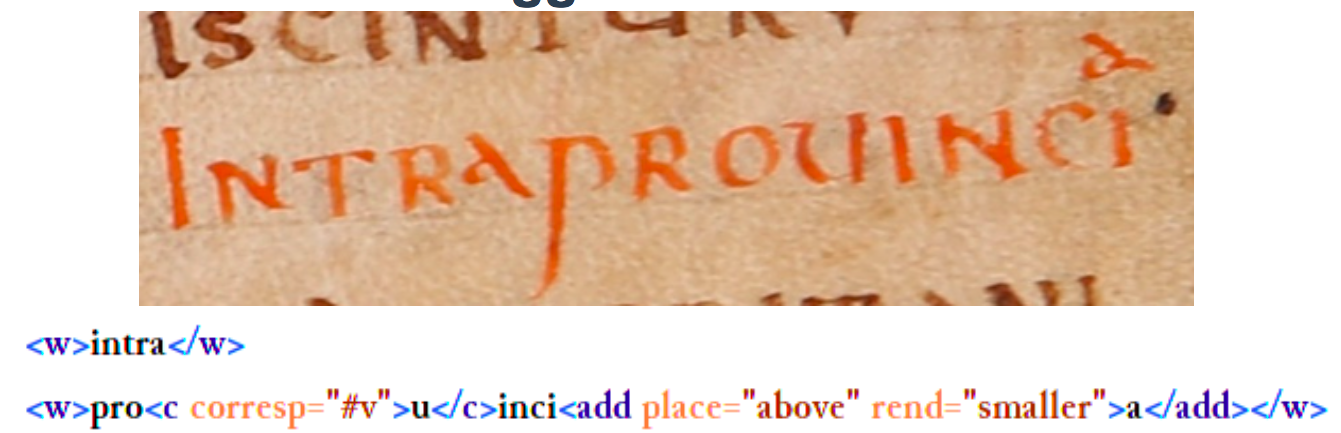
\includegraphics[width=.95\textwidth]{imgs/Aggiunte-1.png}
        \end{center}

    \end{block}
    
\end{frame} 

\begin{frame}
    \frametitle{Elementi interventi editoriali}
    \addtocounter{nframe}{1}
    
   
    \begin{block}{Aggiunte scribali}
        \begin{center}
            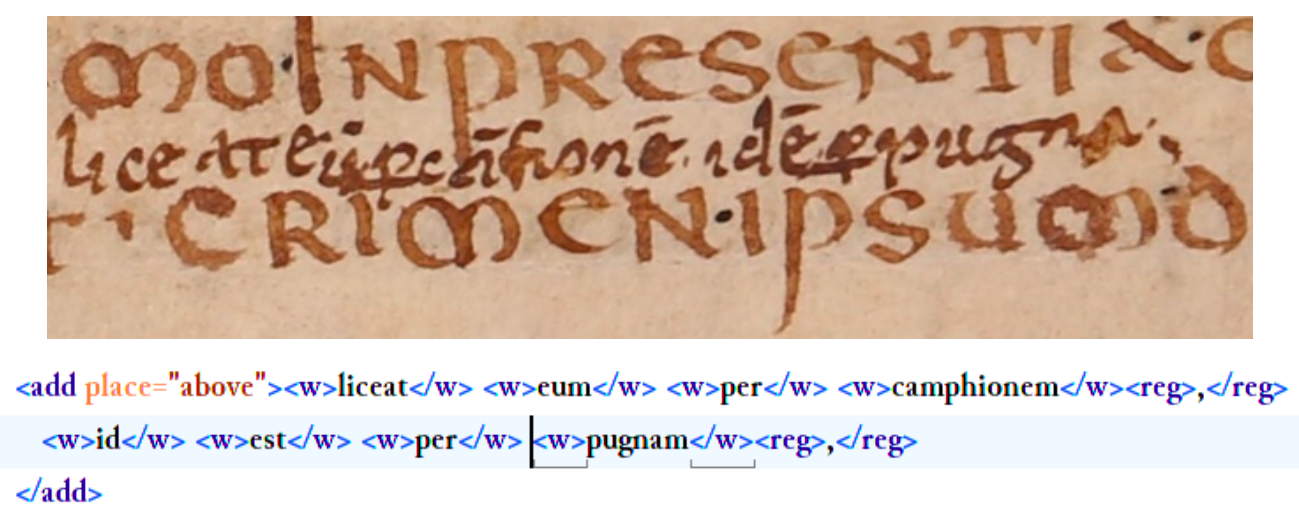
\includegraphics[width=.95\textwidth]{imgs/Aggiunte-2.png}
        \end{center}

    \end{block}
    
\end{frame} 

%%
\begin{frame}
    \frametitle{Elementi interventi editoriali}
    \addtocounter{nframe}{1}
    
    \begin{block}{Cancellature}
        \begin{center}
            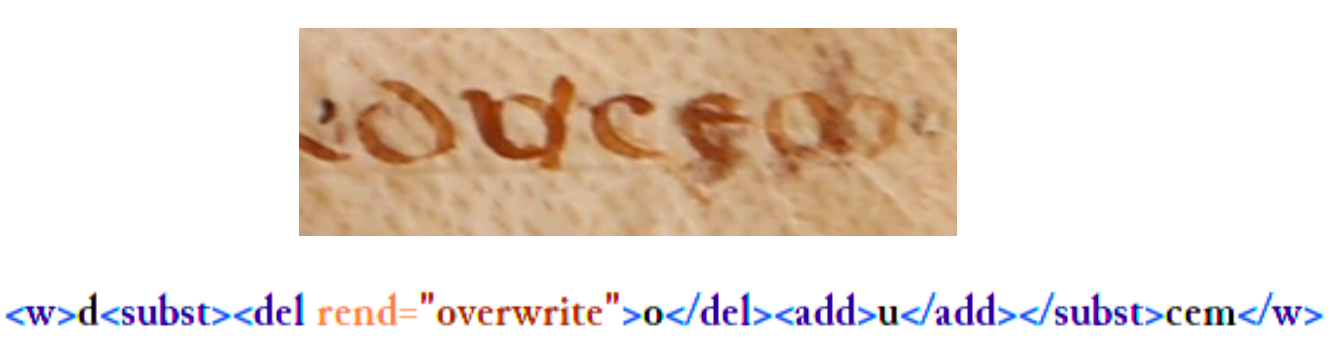
\includegraphics[width=.9\textwidth]{imgs/Cancellature.png}
        \end{center}
    \end{block}
   
    \begin{block}{Cancellature scribali: Dal Vercelli Book}
        \texttt{<del rend="erasure" >ff</del>fore wæron
        <del rend="dot" ><g ref="\#aeligddot"/></del>}
    \end{block}
    
\end{frame} 


\begin{frame}
    \frametitle{Elementi interventi editoriali}
    \addtocounter{nframe}{1}
    
   
    \textit{Abbreviazioni e Espansioni}
        \begin{center}
            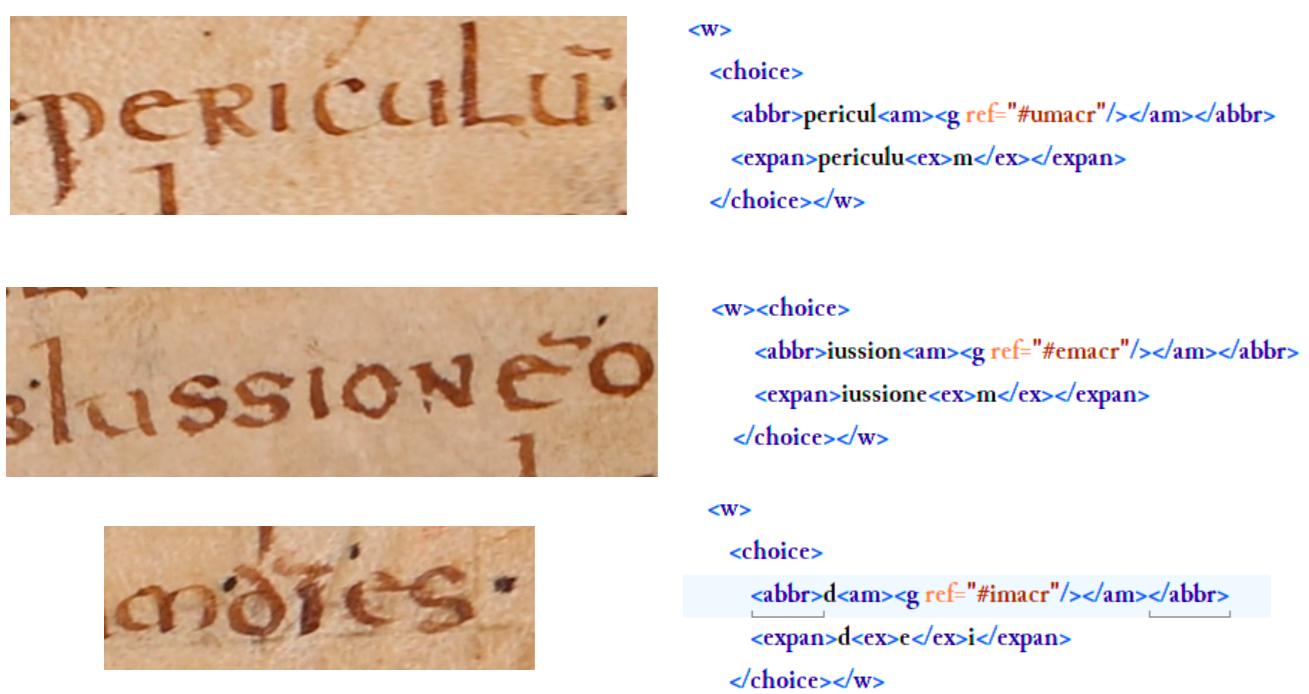
\includegraphics[width=.95\textwidth]{imgs/Abbreviazioni-1.png}
        \end{center}

    
\end{frame}

\begin{frame}
    \frametitle{Elementi interventi editoriali}
    \addtocounter{nframe}{1}
    
   
    \begin{block}{Codifica fenomeni annidati}
        \begin{center}
            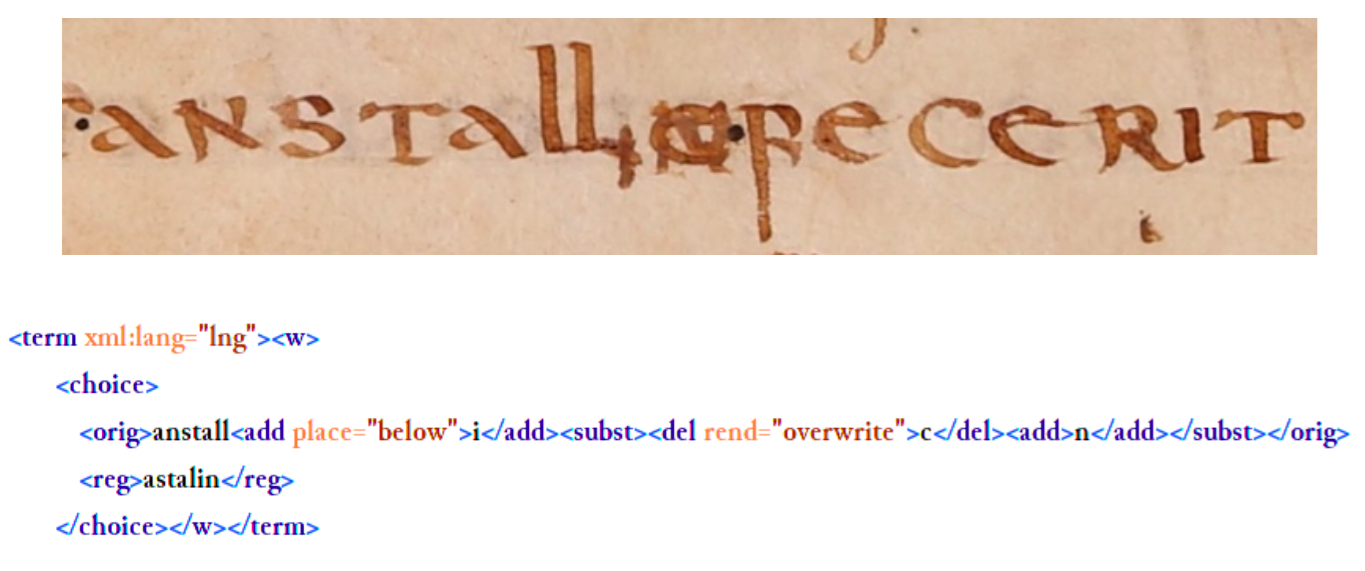
\includegraphics[width=.95\textwidth]{imgs/Aggiunta-cancellatura-regolarizzazione.png}
        \end{center}

    \end{block}
    
\end{frame}

\begin{frame}
    \frametitle{Elementi interventi editoriali}
    \addtocounter{nframe}{1}
    
   
    \begin{block}{Errori Scribali}
        \begin{center}
            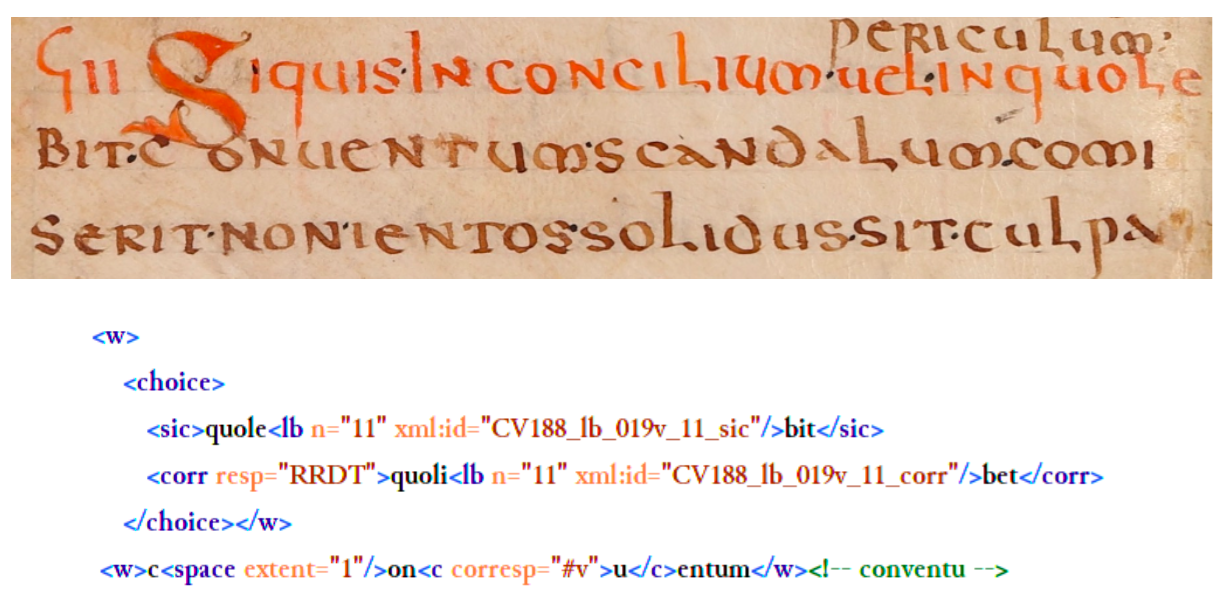
\includegraphics[width=.95\textwidth]{imgs/Correzioni.png}
        \end{center}

    \end{block}
    
\end{frame}

\begin{frame}
    \frametitle{Elementi interventi editoriali}
    \addtocounter{nframe}{1}
        \begin{center}
            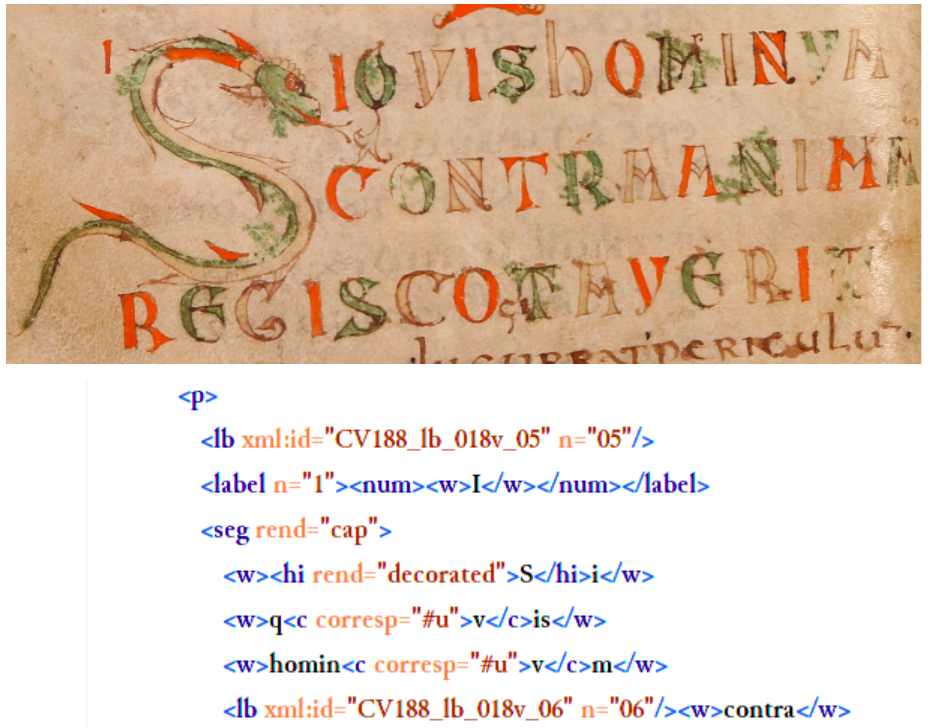
\includegraphics[width=.9\textwidth]{imgs/Decorazioni.png}
        \end{center}
\end{frame}

\begin{frame}
    \frametitle{Elementi interventi editoriali}
    \addtocounter{nframe}{1}
    
    \textit{Marcatura singole parole}
        \begin{center}
            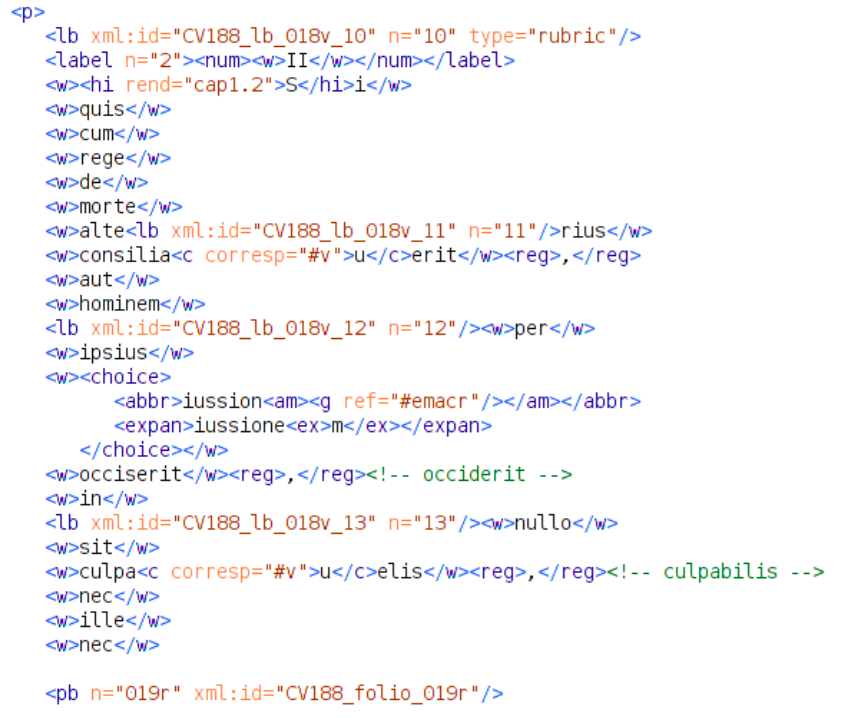
\includegraphics[width=.9\textwidth]{imgs/MarcaturaParole.png}
        \end{center}
    
    
\end{frame}

%% 
\begin{frame}
    \frametitle{Elementi interventi editoriali}
    \addtocounter{nframe}{1}
    
   
    \begin{block}{Esercizio}
        \begin{center}
            Trascrivere e codificare un frammento di lettera di Bellini
            \\(Vincenzo Bellini a Carlo Pepoli, in Puteaux, 26 giugno 1834)
        \end{center}
    \end{block}
    \begin{center}
        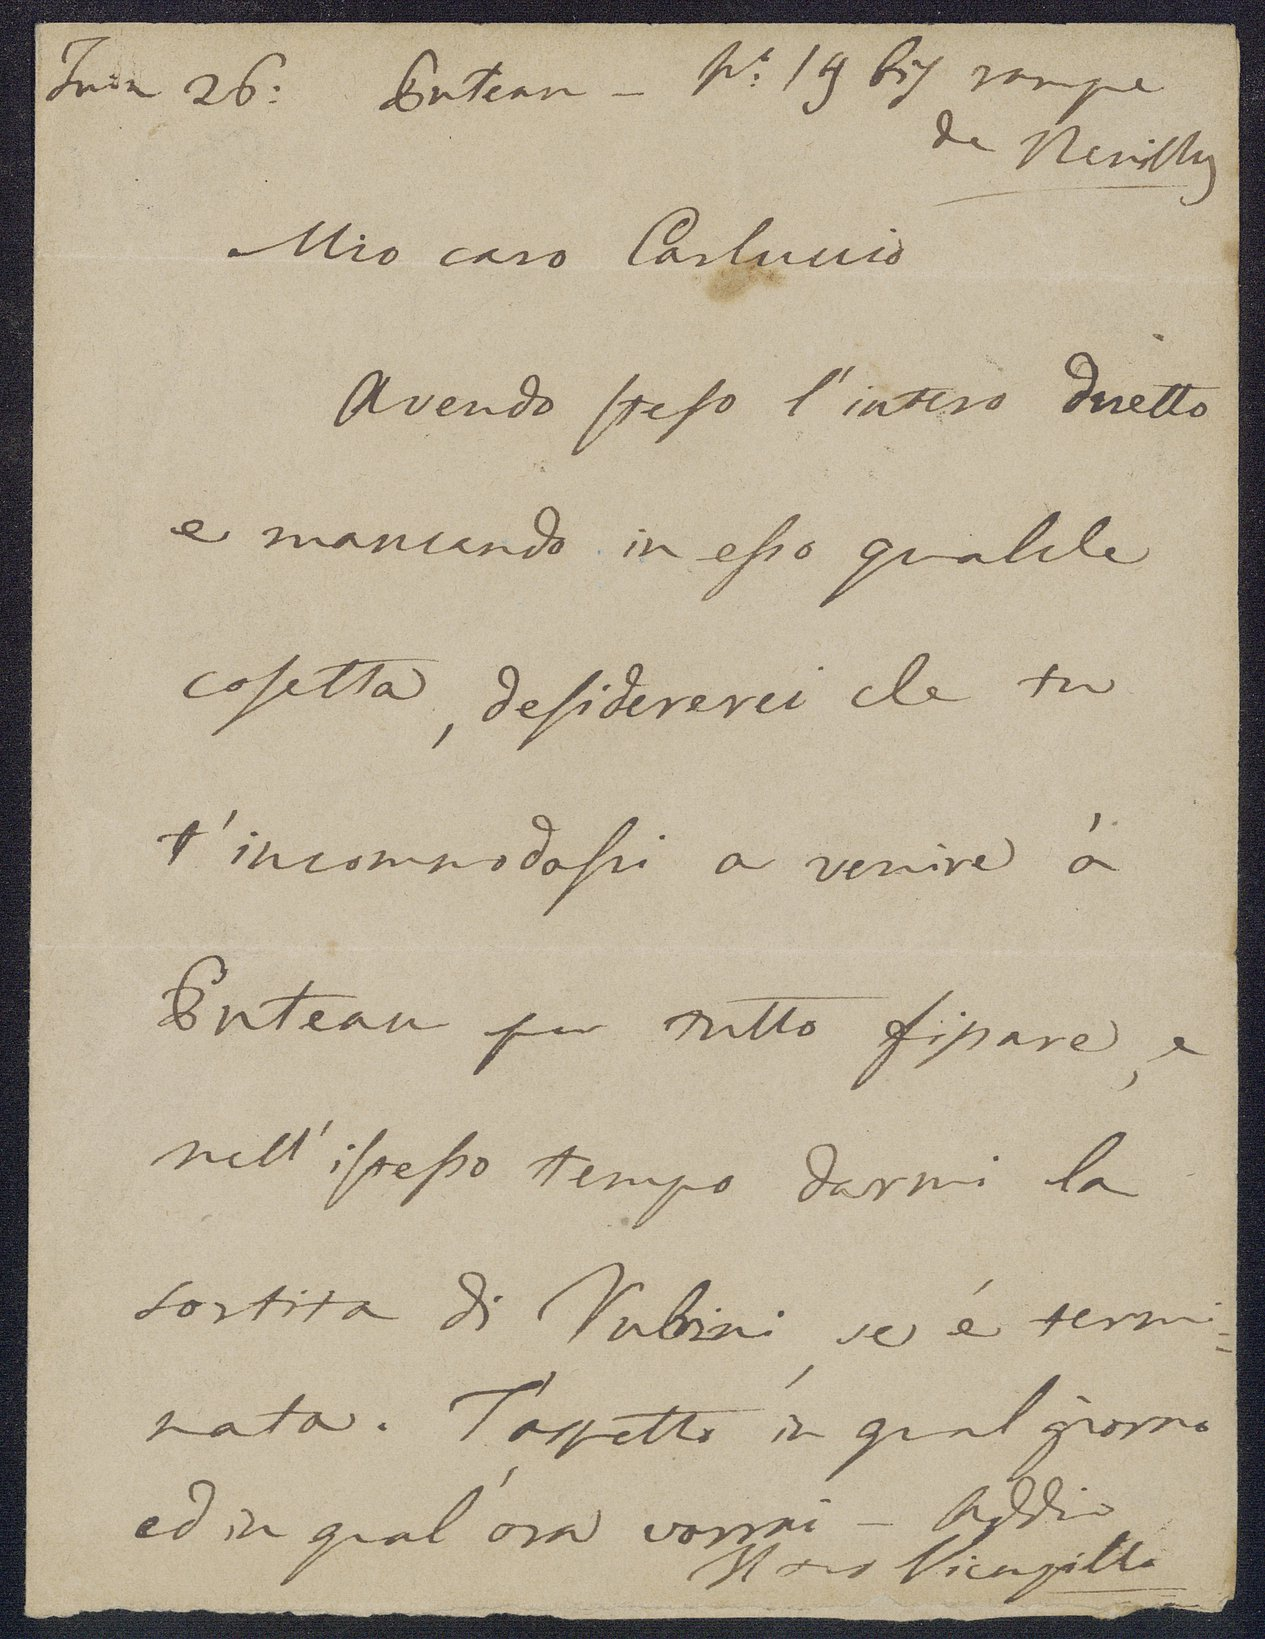
\includegraphics[width=.35\textwidth]{imgs/letteraBellini-1a-LL_1_16.jpg}
    \end{center}
\end{frame}

    
    \section{Elementi facsimile TEI}
    \begin{frame}
    \frametitle{Introduzione}
    \addtocounter{nframe}{1}
    
    %\begin{center}
    %    
\includegraphics[width=.2\textwidth]{../imgs/tei-r.pdf}
    %\end{center}

    \begin{block}{Cos'è la TEI}
        la TEI - \textit{acronimo di Text Encoding Initiative} - rappresenta un punto di riferimento per tutte le iniziative il cui scopo principale è quello di digitalizzare risorse testuali in ambito umanistico per fini di ricerca e di conservazione.
    \end{block}
    
\end{frame}

%%
Tipi di edizione digitale

edizione ipertestuale
prime a essere prodotte, ancora oggi spesso in formato HTML (← TEI XML), formato ideale per e. critiche
distribuzione sul Web (Biblioteca Digitale Italiana) 

facsimile digitale
riproduzione del manoscritto basata su scansione digitale
distribuzione sul Web (Bodleian Library, Oxford)

edizione basata su immagini (image-based digital edition)
il testo dell’edizione (diplomatica, critica) con le immagini del
manoscritto

%%
trascrizione collegata alle immagini del manoscritto serie di funzionalità “standard”:
immagini in formati e/o risoluzioni diverse 
lente d’ingrandimento
evidenziazione dettagli (← restauro digitale) 
motore di ricerca testuale
introduzione paleografica/filologica, 
commento al testo, bibliografia, etc.
(Electronic Beowulf, Vita Nova)

%% 
edizione digitale di un manoscritto

immagini del manoscritto trascrizione del/i testo/i creazione del facsimile digitale collegamento testo-immagine livello di edizione:
edizione diplomatica
edizione diplomatico-interpretativa (edizione critica)
singolo manoscritto = edizione diplomatica e/o interpretativa

%%
livelli di edizione

e. diplomatica: trascrizione del testo di un testimone rispettando la disposizione e la grafia originale, senza nessun tipo di correzione (errori manifesti) o altri interventi editoriali (espansione abbreviazioni)

e. diplomatico-interpretativa: sempre rispettando il testo originale, vengono corretti gli errori più evidenti, regolarizzate certe particolarità ortografiche (suddivisione delle parole), espanse le abbreviazioni, etc.

e. critica: sulla base della collazione di tutte le trascrizioni
dei testimoni viene stabilito lo stemma codicum e si tenta
di ricostruire il testo originale confrontando le varianti dei
testimoni più validi

%%
esempi electronic Beowulf, (variorum), lettere, etc

%%
collegamento mirato (hot-spot): una specifica area dell’immagine viene evidenziata in maniera tale che, interagendo con la stessa, vengono visualizzate delle informazioni quali note editoriali, versione migliorata di un dettaglio, commento al testo, etc.

collegamento generalizzato: tutto il testo dell’edizione viene messo in relazione diretta con le immagini, o parti di immagine, corrispondenti, in modo da poter accedere facilmente alla porzione di immagine corrispondente partendo dal testo, e viceversa

%%
obiettivo: realizzare un collegamento fra testo e immagine in maniera tale che cliccando sul testo viene visualizzata la parte di immagine corrispondente e viceversa

%%
gli schemi di codifica TEI versione P5 (2007) introducono numerosi miglioramenti per quanto riguarda la gestione e trascrizione di manoscritti

%%
tra queste la nuova sezione Digital facsimiles nel capitolo 11 Representation of Primary Sources:
http://www.tei-c.org/release/doc/tei-p5-doc/en/html/PH.html

%%
modulo per la descrizione di manoscritti (10 Manuscript
Description http://www.tei-c.org/release/doc/tei-p5-doc/en/html/MS.html)
nuovo elemento <choice> da usare per le coppie di elementi
di tipo “editoriale”

%%
includendo il modulo transcr nello schema di codifica TEI si rende disponibile un nuovo attributo globale:
@facs (facsimile) points to all or part of an image which corresponds with the content of the element
questo attributo può essere usato in qualsiasi elemento per associare il contenuto dello stesso a un’immagine:
<p n="1" facs="para1.jpg">
<head facs="head.jpg">
<pb facs="page1.jpg"/>

%%
oltre a @facs è necessario usare i nuovi elementi per collegare testo a immagine:
<facsimile> contains a representation of some written source in the form of a set of images rather than as transcribed or encoded text.
<surface> defines a written surface in terms of a rectangular coordinate space, optionally grouping one or more graphic representations of that space, and rectangular zones of interest within it.
@start points to an element which encodes the starting position of the text corresponding to the inscribed part of the surface.
<zone> defines a rectangular area contained within a surface 23 element.

%%
l’elemento <facsimile> è di tipo strutturale e si pone allo stesso livello di <text> o addirittura in alternativa a quest’ultimo
quando il modulo transcr viene aggiunto allo schema di codifica è possibile scegliere fra:
un <teiHeader> e un <facsimile>
un <teiHeader> e un <text>
un <teiHeader>, un <facsimile> e un <text>
questo permette una grande flessibilità:
caso più semplice: facsimile digitale con le immagini del ms
facsimile digitale con trascrizione del testo facsimile digitale con trascrizione e collegamento

%%
<TEI>
 <teiHeader>
  <!­­...­­>
 </teiHeader>
 <facsimile>
  <graphic url="page1.png"/>
  <graphic url="page2.png"/>
  <graphic url="page3.png"/>
  <graphic url="page4.png"/>
 </facsimile>
</TEI>

%%
<TEI>
 <teiHeader>
  <!­­...­­>
 </teiHeader>
 <text>
  <pb facs="page1.png"/>
   <!­­ inserire qui il testo di pagina 1 ­­>
  <pb facs="page2.png"/>
   <!­­ inserire qui il testo di pagina 2 ­­>
 </text>
</TEI>

%%
grazie a un foglio di stile XSLT è possibile generare una pagina HMTL divisa in due riquadri (immagine e testo)
in alternativa è possibile usare un elemento <facsimile> sullo stesso livello di <text>
ma allora sarebbe necessario aggiungere i collegamenti svantaggi di questa soluzione:
nessun collegamento testo-immagine a livello diverso dalla pagina
non è possibile individuare aree particolari delle immagini
i puntatori alle immagini sono sparsi per tutto il documento (a
meno che non si usi un elemento <facsimile>)

%%
la soluzione più efficace è la parallel transcription basata su <facsimile> e <text>
uso di <surface> e <zone> all’interno di <facsimile>
per definire le aree delle immagini
per collegare il testo della trascrizione a tali aree e/o immagini secondarie
le aree delle immagini sono individuate per mezzo di un sistema di coordinate cartesiane registrate come valori dei seguenti attributi di <surface> e <zone>:
ulx, uly coordinate x e y dell’angolo superiore sinistro lrx, lry coordinate x e y dell’angolo inferiore destro

%%
<surface> individua la superficie scritta di un’immagine
<surface ulx="0" uly="0" lrx="400" lry="280"> <graphic url="page1.png"/>
</surface>
può contenere più di un elemento <graphic>
<surface>
<graphic url="page1­highRes.png"/> <graphic url="page1­lowRes.png"/>
</surface>
invece di <graphic> può contenere una o più <zone> <surface> stesso si trova all’interno di <facsimile>

%%
L’elemento <zone>
<zone> definisce una specifica area dell’immagine usando lo stesso sistema di coordinate di <surface>
un’area dell’immagine:
<surface ulx="0" uly="0" lrx="500" lry="321"> <zone ulx="50" uly="20" lrx="400" lry="280">
<graphic url="scrittura.png"/></zone> <note>first page</note>
</surface>
o una porzione più piccola (utile per creare un hot-spot): <zone ulx="120" uly="48" lrx="143" lry="56">
 <graphic url="gloss.png"/>
 <note>Scribe gloss</note>
</zone>

%%
Esempio immagine zone

%%
<facsimile xml:id="imtAnnotatedImage"> <surface>
<graphic height="1797px" url="LindisfarneFol27rIncipitMatt.jpg" width="1266px"/>
<zone lrx="1268" lry="1797" rend="visible" rendition="surface" ulx="0" uly="­4" xml:id="imtArea_0"/>
<zone lrx="1267" lry="450" rend="visible" rendition="zone" ulx="1202" uly="356" xml:id="imtArea_1"/>
<zone lrx="1050" lry="792" rend="visible" rendition="zone" ulx="81" uly="30" xml:id="imtArea_3"/>
<zone lrx="1190" lry="154" rend="visible" rendition="zone" ulx="503" uly="48" xml:id="imtArea_4"/>
<zone lrx="1184" lry="412" rend="visible" rendition="zone" ulx="1116" uly="353" xml:id="imtArea__6"/>
<zone lrx="86" lry="606" rend="visible" rendition="zone" ulx="2" uly="478" xml:id="imtArea_5"/>
<zone lrx="995" lry="366" rend="visible" rendition="zone" ulx="694" uly="321" xml:id="imtArea_6"/>
  </surface>
</facsimile>

%%
Collegare il testo a <surface> e <zone>
per collegare il testo della trascrizione alle aree corrispondenti dell’immagine:
assegnare un identificatore univoco a ciascun elemento del facsimile usando l’attributo xml:id
usare l’attributo facs negli elementi testuali per specificare l’id degli elementi <surface> e <zone> corrispondenti
per collegare le aree delle immagini ai corrispondenti elementi di testo:
assegnare un identificatore univoco a ciascun elemento della trascrizione usando l’attributo xml:id
usare l’attributo start negli elementi <surface> e <zone> per
specificare l’id degli elementi testuali

%%
<text>
 <body>
  <div>
Esempio bidirezionale completo
<pb facs="#page1" n="1" xml:id="page_1"/>
<p>Lorem ipsum ... <gloss facs="#det1">semper</gloss></p> </div>
 </body>
</text>
<facsimile>
<surface xml:id="page1” start="#page_1" ulx="0" uly="0" lrx="500" lry="321">
<graphic url="page1.png”>
<zone xml:id="line1" ulx="50" uly="80" lrx="200" lry="321">
<graphic url="line1.png"/>
<note>First page.</note> </zone>
<zone xml:id="det1" ulx="120" uly="48" lrx="143" lry="56"> <graphic url="gloss.png"/>
<note>Scribe gloss.</note>
  </zone>
 </surface>
36
</facsimile>

%%
Facsimile con embedded transcription un metodo a metà fra facsimile digitale e edizione basata
su immagini è quello della embedded transcription: http://www.tei-c.org/release/doc/tei-p5-
doc/en/html/PH.html#PHZLAB
differenze importanti rispetto a trascrizione parallela basata su <text>:
il testo è considerato “di accompagnamento”, focus sulle immagini (ad esempio disposizione fisica delle parti)
infatti il modello di codifica di <line> è limitato nessun problema di conflitti di gerarchie

%%
Facsimile con embedded transcription uso dell’elemento <sourceDoc> sullo stesso livello
gerarchico e in alternativa a <facsimile> e <text>
uso di <surface> e <zone> in maniera simile a quanto visto in precedenza
<zone> contiene una serie di <line> corrispondenti alle righe di testo
<zone ulx="20" uly="40" lrx="120" lry="180">
   <line>prima riga di trascrizione</line>
   <line>seconda riga di trascrizione</line>
</zone>

%%
Esempio proust

%%
Come inserire le coordinate
domanda n. 1: come trovo i valori delle coordinate?
domanda n. 2: li devo inserire manualmente nei miei documenti TEI XML?
esistono numerosi programmi per calcolare le coordinate:
software di disegno in formato bitmap strumenti per programmatori di siti web
gli strumenti del software EPPT permettono di ottenere i valori delle coordinate e di inserirli automaticamente
software potente, progettato per creatori di edizioni digitali ancora non conforme alla TEI P5 (possibile conversione)

%%
Esempio teizoner

%%



    
    %\section{Elementi di base TEI}
    %% capitoli 3 e 4 delle linee guida e estratti dal libro what is TEI (The structural organization, Varieties of textual structure, parte della TEI cornucopia part 1)
% fare esempio facsimile e codifica dei fenomeni (vedere anche slide del turco e fiormonte-ciotti)
% Elements available in All TEI Documents
% esplicitare le informazioni implicite all'interno del testo.
    
    %\section{Personalizzare TEI}
    %\begin{frame}
	\frametitle{Intro Text Encoding Initiative}
	\framesubtitle{Schemi di codifica TEI – Personalizzare TEI}
	\addtocounter{nframe}{1}

    \begin{block}{Personalizzare TEI}
        Nessun progetto di codifica richiede di utilizzare tutte le specifiche definite dalle linee guida della TEI.
    \end{block}
    \begin{block}{Personalizzare TEI}
        
        La TEI fornisce un insieme specifico di elementi che può essere usato per creare uno schema TEI puntuale e ritagliato sulle specifiche del progetto di codifica in corso.

    \end{block}
    
\end{frame}

% \begin{frame}
% 	\frametitle{Intro Text Encoding Initiative}
% 	\framesubtitle{Schemi di codifica TEI – Personalizzare TEI}
% 	\addtocounter{nframe}{1}

%     \begin{block}{Personalizzare TEI}
%         % The TEI provides a special set of elements which can be used to create such a schema specification.
%         La TEI fornisce un insieme specifico di elementi che può essere usato per creare uno schema TEI puntuale e ritagliato sulle specifiche del progetto di codifica in corso.

%     \end{block}
    
% \end{frame}



\begin{frame}
	\frametitle{Intro Text Encoding Initiative}
	\framesubtitle{Schemi di codifica TEI – Personalizzare TEI}
    \addtocounter{nframe}{1}
    
    \begin{block}{Personalizzare TEI - schemaSpec}
        \texttt{<schemaSpec ident="tei-custom" start="TEI teiCorpus" >}
        \\\texttt{<moduleRef key="analysis" include="interp interpGrp pc s w" />}
        \\\texttt{<moduleRef key="linking" include="anchor seg" />}
        %\texttt{<moduleRef key="tagdocs" include="att code eg gi ident val "/> }
        \\\texttt{<moduleRef key="tei "/> }
        %\texttt{<moduleRef key="textstructure" include="TEI argument back body byline closer dateline div docAuthor docDate docEdition docImprint docTitle epigraph front group imprimatur opener postscript salute signed text titlePage titlePart trailer "/> }
        \\\texttt{</schemaSpec>}
    \end{block}
    \textit{Si selezionano o si escudono gli elementi attraverso gli attributi @\textbf{include} e @\textbf{exclude}}
\end{frame}

\begin{frame}
	\frametitle{Intro Text Encoding Initiative}
	\framesubtitle{Schemi di codifica TEI – Personalizzare TEI}
	\addtocounter{nframe}{1}
    \textit{Modifica agli elementi e attributi dei Moduli}
    \begin{block}{Personalizzare TEI - classSpec}
        \texttt{<classSpec type="atts" ident="att.datable.w3c" module="tei" mode="change" >}
        \\\texttt{<attList> }
        \\\texttt{<attDef ident="notAfter" mode="delete" />}
        \\\texttt{<attDef ident="from" mode="delete" />}
        \\\texttt{<attDef ident="to" mode="delete" /> }
        \\\texttt{</attList>}
        \\\texttt{</classSpec>}
    \end{block}
    
\end{frame}



% ODD document, Selezione dei Moduli per lo schema, nuovi elementi, profilo personalizzato TEI, capitolo 22 delle linee guida (Documentation Elements), capitolo 23 delle linee guida (Using the TEI)


% serious use of the TEI requires careful consideration of exactly which of its elements is appropriate to the of things which the project needs to specify more exactly than the TEI does.


% a document using these elements is provides information for a computer to process along with documentation of that information for a human being to read in a single integrated XML document.

% tei_ all tei_lite epidoc

%% esempio da Exemplars tei_lite.odd
% A quick glance at the XML source code for the TEI Lite ODD shows that it appears to be a typical TEI document

% <schemaSpec ident="tei_lite" start="TEI teiCorpus">
%    <moduleRef key="analysis" include="interp interpGrp pc s w" />
%    <moduleRef key="linking" include="anchor seg" />
%    <moduleRef key=" tagdocs " include="att code eg gi ident val "/> 
%    <moduleRef key="tei "/> 
%    <moduleRef key="textstructure " include="TEI argument back body byline closer dateline div docAuthor docDate docEdition docImprint docTitle epigraph front group imprimatur opener postscript salute signed text titlePage titlePart trailer "/> 
% </schemaSpec>


% TEI currently defines 22 modules
% foto con la tabella

% definizione degli elementi, degli attributi, dei datatype e dei valori di default 




%% esempio epidoc

% <elementSpec   ident="div"   mode="change"   module="textstructure">
%    <attList>
%        <attDef ident="type"     mode="replace"     usage="req">
%            <valList type="closed">
%                <valItem ident="apparatus">
%                    <desc>to contain apparatus criticus or textual notes</desc>
%                    </valItem>
%                    <valItem ident="bibliography">
%                        <desc>to contain bibliographical information, previous publications,            etc.
%                        </desc>
%                        </valItem>
%                        <valItem ident="commentary">
%                            <desc>to contain all editorial commentary, historical/prosopographical            discussion, etc.</desc>
%                            </valItem>
%                            <valItem ident="edition">
%                                <desc>to contain the text of the edition itself; may include multiple            text-parts
%                                </desc>
%                                </valItem>
%                                <valItem ident="textpart">
%                                    <desc>used to divide a div[type=edition] into multiple parts (fragments,            columns,
%                                        faces, etc.)</desc>
%                                    </valItem>
%                                    <valItem ident="translation">
%                                        <desc>to contain a translation of the text into one or more modern            languages
%                                        </desc>
%                                        </valItem>
%                                       </valList>
%        </attDef>
%    </attList>
% </elementSpec>

% esempio aggiunta nuovo elemento: <SpaciesName />

%  Choices can be made explicit in a customized schema, and hence tell us which of the many very different approaches to tagging an individual’s name has been adopted in a given set of documents.


    
    \section{Conclusioni}
    %%
\begin{frame}
    \frametitle{Introduzione}
    \addtocounter{nframe}{1}
    
    %\begin{center}
    %    
\includegraphics[width=.2\textwidth]{../imgs/tei-r.pdf}
    %\end{center}

    \begin{block}{Cos'è la TEI}
        Le nuove caratteristiche degli schemi TEI P5 offrono un’ottima base per edizioni digitali complesse con collegamento testo-immagine
    \end{block}
    
\end{frame}



%%
\begin{frame}
    \frametitle{Conclusioni: Editioni Digitali}
    \addtocounter{nframe}{1}
    
    %\begin{center}
    %    
\includegraphics[width=.2\textwidth]{../imgs/tei-r.pdf}
    %\end{center}

    \begin{block}{Edizioni digitali scientifiche}
        \begin{itemize}
            \item elementi contenuti nei moduli di base
            \item elementi del modulo di descrizione dei manoscritti
            \item elementi del modulo di trascrizione delle fonti primarie
            \item elementi del modulo di apparato critico
            \item elementi del modulo di gestione di caratteri non standard
        \end{itemize}
    \end{block}
    
\end{frame}

%%

\begin{frame}
    \frametitle{Conclusioni: Edizioni Digitali}
    \addtocounter{nframe}{1}
    
    %\begin{center}
    %    
\includegraphics[width=.2\textwidth]{../imgs/tei-r.pdf}
    %\end{center}

    \begin{block}{elementi per interventi editoriali:}
        \texttt{<abbr> <expan>, <orig> <reg>, <sic> <corr>, <subst>
        <gap/>, <supplied>, <unclear>, <damage>}
    \end{block}

    \begin{block}{strutturali specifici:}
        \texttt{<gb/>, <line>}
    \end{block}
    
\end{frame}


%%
\begin{frame}
    \frametitle{Conclusioni: Edizioni Digitali}
    \addtocounter{nframe}{1}
    
    %\begin{center}
    %    
\includegraphics[width=.2\textwidth]{../imgs/tei-r.pdf}
    %\end{center}

    \begin{block}{Elementi di intervento editoriali}
        \begin{itemize}
            \item \texttt{<damage>} marca la parte di testo danneggiata
            \item[] non proprio “intervento editoriale” ma spesso usato contestualmente con \texttt{<gap/>,  <unclear> e <supplied>}
            \item \texttt{<supplied>} testo inserito dal curatore perché l’originale è mancante o illeggibile
        \end{itemize} 
    \end{block}
\end{frame}

\begin{frame}
    \frametitle{Conclusioni: Edizioni Digitali}
    \addtocounter{nframe}{1}
    
    %\begin{center}
    %    
\includegraphics[width=.2\textwidth]{../imgs/tei-r.pdf}
    %\end{center}

    \begin{block}{Elementi di intervento editoriali: esempio}
        \texttt{<l n="1" >Nel mezzo del cammin di nostra vita</l>}
        \\\texttt{<l n="2" ><damage agent="fire" extent="1line" ><unclear>Mi ritrovai</unclear> <supplied reason="illegible" resp="rrdt" >per una selva oscura,</supplied></damage></l>}
        \\\texttt{<l n="3" >Ché la diritta via era smarrita</l>}
    \end{block}
\end{frame}

%%
\begin{frame}
    \frametitle{Conclusioni: Edizioni Digitali}
    \addtocounter{nframe}{1}
    
    %\begin{center}
    %    \includegraphics[width=.2\textwidth]{../imgs/tei-r.pdf}
    %\end{center}

    \begin{block}{Elementi di intervento editoriale}
        \begin{itemize}
            \item \texttt{<subst>} raggruppa una cancellazione e un’aggiunta scribale per rendere evidente che si tratta di una sostituzione
            \item[] Stessa semantica funzionale di \texttt{<choice>}
        \end{itemize}
    \end{block}

\end{frame}

%%
\begin{frame}
    \frametitle{Conclusioni: Edizioni Digitali}
    \addtocounter{nframe}{1}
    
    %\begin{center}
    %    \includegraphics[width=.2\textwidth]{../imgs/tei-r.pdf}
    %\end{center}

    \begin{block}{Elementi di intervento editoriale}
        \texttt{<l n="1" >Nel mezzo del cammin di nostra vita</l> }
        \\\texttt{<l n="2" >Mi ritrovai }
        \\\texttt{<subst>}
        \\\texttt{<del>pir</del>}
        \\\texttt{<add>per</add>}
        \\\texttt{</subst>}
        \\\texttt{una selva oscura,</l>}
        \\\texttt{<l n="3" >Ché la diritta via era smarrita</l>}
    \end{block}
    
\end{frame}


%%

\begin{frame}
    \frametitle{Conclusioni: Edizioni Digitali}
    \addtocounter{nframe}{1}
    
    %\begin{center}
    %    \includegraphics[width=.2\textwidth]{../imgs/tei-r.pdf}
    %\end{center}

    \begin{block}{Edizione image-based: Elementi strutturali}
        \begin{itemize}
            \item \texttt{<gb/>} \textbf{gathering begins} 
            \item[] marca il punto in cui si presenta un nuovo fascicolo all’interno di un manoscritto
            \item \texttt{@type:} classificazione in base al tipo
            \item \texttt{@n:} numero progressivo
        \end{itemize}
    \end{block}
\end{frame}

\begin{frame}
    \frametitle{Conclusioni: Edizioni Digitali}
    \addtocounter{nframe}{1}
    
    %\begin{center}
    %    \includegraphics[width=.2\textwidth]{../imgs/tei-r.pdf}
    %\end{center}

    \begin{block}{Edizione image-based: Elementi strutturali}
        \begin{itemize}
            \item \texttt{<line> }
            \item[] trascrizione di una riga del foglio del manoscritto 
            \item[] \textbf{può essere contenuto solo da \texttt{<surface> e <zone>}!}
            \item per le righe di testo da inserire all’interno di \texttt{<text>} è sempre necessario usare \texttt{<lb/>}.
        \end{itemize}
    \end{block}
\end{frame}

%%
\begin{frame}
    \frametitle{Conclusioni: Edizioni Digitali}
    \addtocounter{nframe}{1}
    
    %\begin{center}
    %    \includegraphics[width=.2\textwidth]{../imgs/tei-r.pdf}
    %\end{center}

    \begin{block}{Elementi per interventi editoriali}
        A causa della relativa complessità di codifica di edizioni digitali image-based è preferibile usare strumenti software per facilitare la creazione di un facsimile digitale
    \end{block}

    \begin{block}{strutturali specifici}
        Manca però ancora uno strumento/funzione per collegare le immagini annotate al testo della trascrizione
    \end{block}
\end{frame}


    
    \end{document}